\documentclass[12pt]{article}

\title{Cosmic dark matter density and the tessellated 3-sphere}
\author{S. Halayka -- sjhalayka@gmail.com}
\date{\today}

\usepackage{listings}
\usepackage{cite}
\usepackage{xcolor}
\usepackage{graphicx}
\usepackage{setspace}
\usepackage{amsmath}
\usepackage{url}
\usepackage[margin=1in]{geometry}
\begin{document}



 
\maketitle

\begin{abstract}
The tessellation of space is considered for both the 2-sphere and the 3-sphere.
As hypothesized in an earlier work, it is found that there is a dark matter density $\Omega_{DM} = 0.284 \pm 0.137$ associated with the curvature of the 3-sphere.
\end{abstract}



\section{Introduction}

Questions arise in physics as to the origin of various measured norms and natural constants.  
Here we examine a construction where tilings of the 2-sphere and 3-sphere are contrasted, and generalized tessellations used as probes are found to produce such a number - the dark matter density.
The approach of using tessellation to model spacetime and its evolution was already covered by Misner, Thorne, and Wheeler back in 1973.
Since that time; a number of Quantum Gravity theories have appeared including CDT (Causal Dynamical Triangulations) in which the nature and evolution of spacetime are probed via tessellations.
This paper explores how, using arbitrary extents, a number arises in the ratio between sphere tilings that matches astrophysical observations.



\section{Curvature and dark matter density}

For a method of calculating the curvature $K$ of triangle meshes and tetrahedron meshes, please see \cite{halayka}.
Unlike in \cite{halayka}, the tessellations in this paper will rely on pseudorandomly placed vertices, rather than the vertices placed by Marching Cubes and Marching Hypercubes.
Also unlike in \cite{halayka}, we will not be compensating for the variation in simplex extent (e.g. do nothing special even where there are sliver simplices).
In effect, the calculation of the curvature is as simple as possible.
The vertex count is $N$.

On one hand, it is found that for a tessellated 2-sphere, the local curvature vanishes when the tessellation is made up of finer and finer triangles.
That is, the more vertices $N$ used in the tessellation, the less the local curvature is:
\begin{equation}
\lim_{N \to \infty} K(N) = 0.0.
\end{equation}

On the other hand, it is found that for a tessellated 3-sphere, the local curvature does {\it not} vanish when the tessellation is made up of finer and finer tetrahedra.
The curvature settles around
\begin{equation}
\lim_{N \to \infty} K(N) = 0.284 \pm 0.137.
\end{equation}
This is in line with the dark matter density measure $\Omega_{DM}$ used in the various $x$CDM models.
If this is not merely a coincidence, then this is direct evidence of the discrete nature of space, based on a few simple, first principles -- at least on the computer, anyway.

Fig. 1 shows a tessellated 2-sphere, with pseudorandomly placed vertices, as well as nearest neighbour edges.\footnote{... thus forming a convex hull; a Delaunay triangulation.}
See Fig. 2 for a 3-sphere nearest neighbour edge length histogram, where vertex count $N = 1,000,000$.
Also see Table 1 for a list of properties of the histograms where the vertex count $N$ is variable.
A C++ code for generating the tessellated 3-sphere\footnote{... also forming a convex hull; a Delaunay tetrahedralization.} can be found at \cite{halayka2}.
The code requires the qhull executables for mesh generation.



\section{Conclusion}

There exists an inherent curvature in the tessellated 3-sphere, which we use as a toy model for the Universe.
This curvature matches the dark matter density of the actual Universe.
As far as we know, this is a novel finding.



\section { Acknowledgements }
Thank you to Jonathan J. Dickau for assistance with writing the Introduction and Conclusion sections.




\begin{figure} 
\centering
  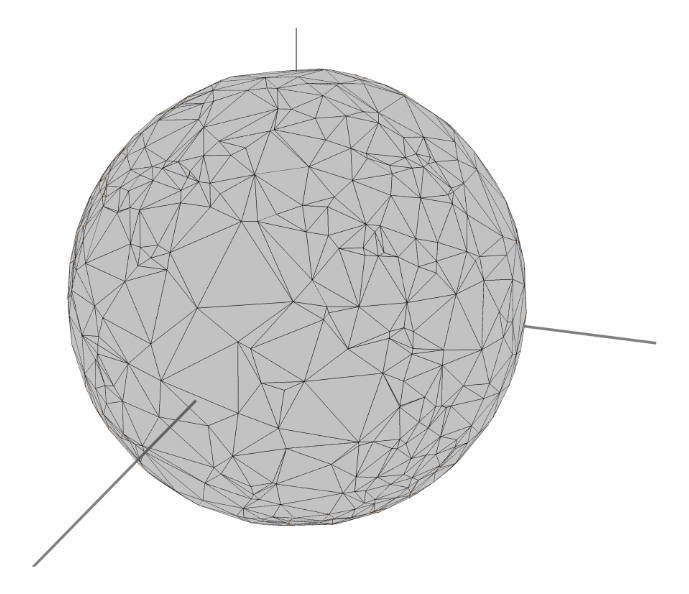
\includegraphics[width = 3 in]{2sphere.png}	
  \caption{Tessellated 2-sphere, where there are $N = 1,000$ pseudorandomly placed vertices.
The 2D triangles exist in 3D space.
Accordingly, for a tessellated 3-sphere, the 3D tetrahedra exist in 4D space. }
\end{figure}





\begin{figure} 
\centering
  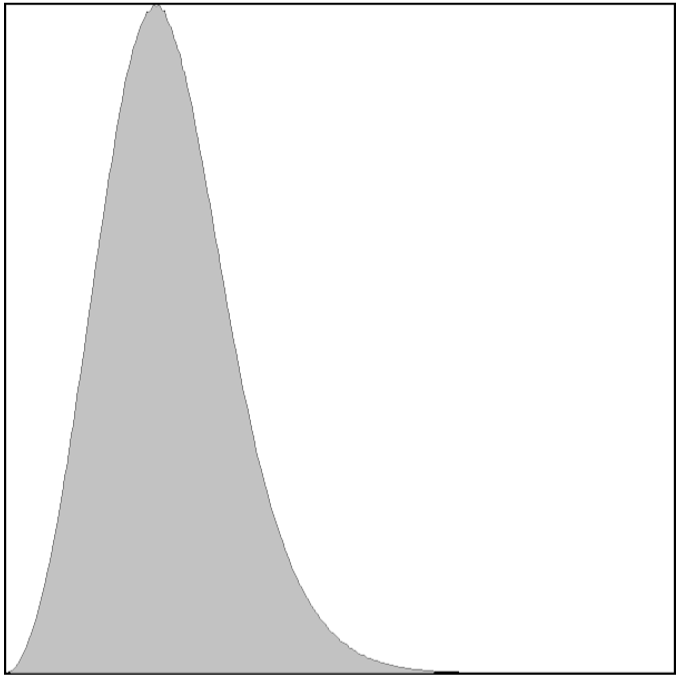
\includegraphics[width = 3 in]{histogram_1000000.png}	
  \caption{3-sphere nearest neighbour edge length histogram, where vertex count $N = 1,000,000$. Max $= 0.0565194$, mode $= 0.012455$, curvature $K = 0.28452$.}
\end{figure}





\begin{table}
\centering
\begin{tabular}{|l|l|l|l|l|}
\hline
$N$ & $K$ & Max & Mode & Max / Mode  \\ 
\hline
\hline
1,000
& 
0.29473
& 
0.405105
&
0.132555
&
3.05612
\\
\hline
10,000
& 
0.28821
& 
0.215664
&
0.0619268
&
3.48256
\\
\hline
100,000
& 
0.28413
& 
0.113452
&
0.0268951
&
4.21831
\\

\hline
1,000,000
& 
0.28452
& 
0.0565194
&
0.012455
&
4.53788
\\


\hline



\end{tabular}
\caption{Properties of the histograms where vertex count $N$ is variable.}
\end{table} 




\begin{thebibliography}{9}
\bibitem{mtw} Misner, Thorne, Wheeler. (1973) "Gravitation"
\bibitem{cdt} Ambjorn, Jurkiewicz, Loll. (2006) "Quantum Gravity, or The Art of Building Spacetime" \\ \url{https://arxiv.org/abs/hep-th/0604212}
\bibitem{nicolson} Nicolson. (2007) "Dark Side of the Universe: Dark Matter, Dark Energy, and the Fate of the Cosmos"
\bibitem{binney} Binney, Merrifield. (1998) "Galactic Astronomy"
\bibitem{binney2} Binney, Tremaine. (2008) "Galactic Dynamics"
\bibitem{halayka} Halayka. (2020) "The curvature and dimension of a closed surface" \\ \url{https://vixra.org/abs/1812.0423}
\bibitem{halayka2} Halayka. (2020) "3-sphere Universe C++ code" \\  \url{https://github.com/sjhalayka/4d_universe}

\end{thebibliography}



\end{document}









